\documentclass[review]{elsarticle}

\usepackage{lineno, hyperref}
% \usepackage[hyperfootnotes=false]{hyperref}
\usepackage{array, pbox}
\usepackage{mathtools}
\usepackage{caption}
\usepackage{graphicx}
\usepackage{subcaption}
\usepackage{CJKutf8}
\usepackage[page, title]{appendix}
% \usepackage{tablefootnote}
\usepackage{threeparttable}
\usepackage{etoolbox}
\appto\TPTnoteSettings{\footnotesize}
\usepackage[bottom]{footmisc}
\usepackage{siunitx}

%to have numbered 4th level sections 1.1.1.1
\setcounter{tocdepth}{4}
\setcounter{secnumdepth}{4}

% to remove period in 4th level sections 1.1.1.1
\makeatletter
\def\els@aparagraph[#1]#2{\elsparagraph[#1]{#2}}
\def\els@bparagraph#1{\elsparagraph*{#1}}
\makeatother
% to enter a newline after 4th level sections
\newcommand{\myparagraph}[1]{\paragraph{#1}\mbox{}\smallskip}


\modulolinenumbers[5]

\journal{Tourism Management Perspectives}

%%%%%%%%%%%%%%%%%%%%%%%
%% Elsevier bibliography styles
%%%%%%%%%%%%%%%%%%%%%%%
%% To change the style, put a % in front of the second line of the current style and
%% remove the % from the second line of the style you would like to use.
%%%%%%%%%%%%%%%%%%%%%%%

%% Numbered
%\bibliographystyle{model1-num-names}

%% Numbered without titles
%\bibliographystyle{model1a-num-names}

%% Harvard
%\bibliographystyle{model2-names.bst}\biboptions{authoryear}

%% Vancouver numbered
%\usepackage{numcompress}\bibliographystyle{model3-num-names}

%% Vancouver name/year
%\usepackage{numcompress}\bibliographystyle{model4-names}\biboptions{authoryear}

%% APA style
\bibliographystyle{model5-names}\biboptions{authoryear}

%% AMA style
%\usepackage{numcompress}\bibliographystyle{model6-num-names}

%% `Elsevier LaTeX' style
% \bibliographystyle{elsarticle-num}
%%%%%%%%%%%%%%%%%%%%%%%

\begin{document}

\begin{frontmatter}

\title{Quantitative ranking of satisfaction and dissatisfaction factors based on text mining of online reviews from Chinese and English speaking tourists visiting Japan}

%% or include affiliations in footnotes:
\author[gidai]{Elisa Claire Alemán Carreón
\corref{mycorrespondingauthor}}
\ead{s153400@stn.nagaokaut.ac.jp}
% \orcid{0000-0002-6437-0866}

\author[gidai]{Hirofumi Nonaka}
\ead{nonaka@kjs.nagaokaut.ac.jp}

\author[nagasaki]{Toru Hiraoka}
\ead{hiraoka@sun.ac.jp}

\address[gidai]{Nagaoka University of Technology, Nagaoka, Japan}
\address[nagasaki]{University of Nagasaki, Nagasaki, Japan}

\cortext[mycorrespondingauthor]{
Corresponding author%: \\
% Elisa Claire Alemán Carreón \\
% Mailing Address: P.C. 940-2033, Ribbon Nagaoka B104, 1128-3 Kaminozoki-machi, Nagaoka, Niigata, Japan \\
% Cell Phone: 080-9869-4756 \\
}

\begin{abstract}
Recently, there has been a boom in international tourism in Japan, where particularly Chinese tourists are increasing rapidly, among other international tourists. Because of its effect on the Japanese economy, there is a need for the use of newer research tools that are cost and time effective and use online reviews, which increasingly affect sales and the influx of customers. Using machine learning, we determined keywords representing satisfaction and dissatisfaction factors from Chinese and English online reviews of Japanese hotels in the portal sites \textit{Ctrip} and \textit{TripAdvisor}. We identified that Chinese customers react positively to included breakfasts and big rooms, and are unsatisfied with the pricing of the hotel. We also found English speaking customers dislike pricey hotels and have a high dislike for dirty rooms, stains, and cigarette smell, and that they mainly focus positively on staff, cleanliness, and transportation availability.

\medskip
\noindent\it{Highlights}
\begin{itemize}
    \item Chinese customers tend to prefer included breakfasts, and rooms that are big and clean.
    \item Across all hotel prices, unsatisfied Chinese customers focus on the pricing of the hotel.
    \item English speaking customers are satisfied with the staff, cleanliness, and transportation availability.
    \item English speaking customers dislike pricey hotels and have a high dislike for dirty rooms and cigarette smell.
\end{itemize}

\end{abstract}

\begin{keyword}
Entropy\sep Sentiment Analysis\sep Hotels and Lodging\sep Support Vector Machine\sep Chinese\sep Satisfaction and Dissatisfaction
\end{keyword}

\end{frontmatter}

\section{Introduction}\label{intro}

The population of Chinese tourists has recently increased significantly worldwide over the years. This increase has led to a significant impact on several industries over the world, most directly the hotel industry, as their customer bases changed. In addition to this impact on business, there is a current increase in academic research across the world about Chinese tourist populations \cite[][]{sun2017}. Particularly in Japan, however, international tourism has been increasingly exerting a stronger influence in the economy \cite[][]{Jones2009}. There were notable increases in the Chinese tourist population in Japan of 107.3\% from 2014 to 2015, and a total number of tourists of \num[group-separator={,}]{6372948} in 2016 \cite[][]{jnto2017}. This increase in international tourism creates a need for cross-language, cost and time effective market research tools. In the hospitality industry, where language barriers are a constant problem, there are difficulties and costs when attempting to understand the needs of their customer base. 

Until recent years, most of these market studies are performed based on the results of surveys or interviews. Currently, however, there are data mining and text mining techniques which potentially have the advantage over surveys and interviews. During recent years, several studies have successfully proved the validity and potential of using text and data mining analysis in the business management field. A study classified different kinds of Social Media posts and customer response from several U.S. pizza selling companies \cite[][]{he2013}. Another study ranked products by using online reviews and sentiment analysis \cite[][]{liu2017149}, while another used them to predict product sales \cite[][]{fan201790}. Other uses for text mining techniques include patent document analysis, as was done in a study on patent scoring \cite[][]{nonaka2014}, and another on the extraction of technological terminology in patents \cite[][]{nonaka2012}. It has also been used in the tourism and hospitality field to predict hotel demand by using web traffic data \cite[][]{yang2014} or to make recommender systems \cite[][]{loh2003}. Data mining and text mining techniques can not only cheaply and quickly gather tens of thousands if not more samples, but the source of this extensive amount of information also can be thought to be unaltered by human intervention in any part of the data extraction process. 

An important benefit of using data and text mining in the hospitality field is that because of the current behavior of the customers in the information age, where the searching, choosing and booking process involves reading online reviews, and where customers write online reviews depending on their satisfaction or dissatisfaction. Previous studies have found that there is a correlation between prominent reviews and sales figures \cite[][]{basuroy2003, ye2009}. There are also studies showing the direct impact of online hotel reviews on consumer consideration, that is, the decision process of many customers is affected either positively or negatively because of the reviews, with a stronger impact for lesser known hotels \cite[][]{vermeulen2009}. Online reviews give researchers access to large databases of unfiltered customers opinions without the need to ask directly via surveys or interviews, and they also provide availability of data from tourists writing in many languages. It is because of the important impact the hotel reviews have on consumers, and because of the highly polarized emotional content these reviews hold that we have decided to use this data for analysis.

Many researchers have focused on studying the level of satisfaction of customers for predefined factors \cite[e.g.][]{balbi2018, kim2017362, truong2009, wu2009, shanka2004, kozak2002}, while others focus on motivation, choice or behavior \cite[e.g.][]{romao2014, dongyang2015}. However, most of the studies rely on making inferences about the larger population based on predefined factors, instead of extracting the factors directly from the data without human intervention. Not only that but when examining international tourism, they are limited by language barriers. In our study, we aim to use the benefits of online reviews to mathematically extract the answer to these questions in a manner that doesn't rely on understanding the language to expand it further to a larger corpus. In addition, while most studies with text mining techniques and sentiment analysis techniques focus on either relevant topics or the sentiment value of reviews, this study merges both techniques to find the relevant topics and their ties to each emotional response.

In our study, we extracted satisfaction and dissatisfaction keywords and analyzed the needs of Chinese and English speaking customers of Japanese Hotels. We chose this combination of population and destination because we aim to apply machine learning techniques to overcome language barriers on a large scale. The extracted keywords are the key to researching which topics and in what order of priority the Chinese tourist and English speaking tourist populations consider when they write their reviews. This is, of course, valuable information for making business management decisions from the point of view of the hotel industry companies. Knowing which topics are not only largely discussed, but those that are most related to customer satisfaction and dissatisfaction, a company can improve customer service or facilities to increase profit. Using the methodology detailed in this study, such knowledge can become available to other researchers and companies by applying it in different environments.

\section{Research objective}\label{research_objective}

The objective of this study is to determine the factors influencing the satisfaction or dissatisfaction of Chinese customers as well as studying English speaking customers of Japanese Hotels because of the language barrier that can be studied and the economic weight that these customers represent. These satisfaction and dissatisfaction factors can become the focal point for making improvements in tourism and service industries, increase the satisfaction of customers, and influence newer customers to write more satisfied online reviews that will in turn increase sales and attract new customers. 

We propose to avoid language barrier limitations by using a process that is based on probability distributions and automatic algorithms, and that is not dependent on language-specific methodologies that limit its application in other environments. To do this, we propose to use a supervised machine learning methodology to be trained on the emotional classification of a sample online review texts and use it not only to classify other texts further but to analyze the weight towards classification that certain keywords hold in that trained machine. Furthermore, we also analyze the relevance of these keywords in different hotel price brackets to observe potential differences. 

\section{Related work}\label{relatedwork}

In the hospitality field, satisfaction, motivation, and behavior have been studied for a long time using surveys \cite[e.g.][]{truong2009, wu2009, shanka2004, kozak2002, romao2014, dongyang2015, chan201518}. More recently, studies have used big data in the hospitality industry \cite[e.g.][]{yang2014, loh2003}, as well as data mining tools to analyze hotel reviews \cite[e.g.][]{alsmadi2018, browning2013, xiang2010}. However, most of these studies focus on either the sentiment classification without analyzing the relevant words tied to those sentiments, or they study the most relevant words without taking the emotions they largely represent into account. Other studies focus on review helpfulness \cite[][]{ren2019}; while others focus on summarization of reviews into smaller text \cite[e.g.][]{hu2017436, amplayo201754}. There has not been yet a study that focuses on the conceptual words that are tied with the satisfaction or dissatisfaction of the userbase. For example, one study used a tool called “Word Cloud” to extract frequently used words inside the reviews which were considered important topics of concern to consumers \cite[][]{hargreaves2015}. However, the sentiment analysis is done at a hotel level, instead of a word level, so it is difficult to determine which topics are perceived positively or negatively. Another study used a heuristic frequency analysis to determine guest experience topics \cite[][]{xiang2015}. However, this study doesn't deterministically show which topics are directly tied with satisfaction and dissatisfaction or the ranking order in which they do.

On the other hand, \cite{zhang2011} performed a market analysis based on the sentiment analysis of product reviews using a Chinese sentiment dictionary called HowNet. The problem with using HowNet as a sentiment dictionary is that the words are classified based on ontology \cite[][]{huang2008}, where emotional words are usually those that describe emotions, such as “angry”, “anger”, “happiness”, “content”. While these words represent the emotions themselves, in an online review, it is unlikely that the general population writes their emotions explicitly; instead, it is more likely that words that do not describe the emotion but are intrinsically emotionally fueled are used. For example, one would not write “I am happy with the size of the room and the service”; instead what would be natural is “The room had lots of space for our luggage and the staff was friendly”. HowNet is not able to determine that “space” is tied to positive emotions and that “staff” is being praised by the use of “friendly” in the sentence. These non-emotional words are directly representing the emotion of satisfaction or dissatisfaction in the online review. Now, in turn, this study methodology focuses on the influence of each word and their rank of importance in relation to the satisfaction or dissatisfaction expressed by the user, clearly defining not only their emotion but also the specific needs of Chinese customers in a concrete way.

There have been previous attempts at understanding the factors leading to satisfaction and dissatisfaction with text and data mining techniques as well. One study used a text-link analysis to understand which pairs of words were used more in positive or negative reviews \cite[][]{berezina2016}. However, the conclusions of this study are limited to their sample of manually classified 20 reviews, so it is difficult to extrapolate it to a larger population of reviews. Another study manually extracted factors that could lead to satisfaction or dissatisfaction from a sample and then continued to study the statistical differences between them in that sample \cite[][]{zhou2014}. However, this is limited to their manually defined factors and that there are no further analyses to a larger number of online reviews because of language barriers. Another study used heuristic language-specific parsing algorithms to determine the frequency of words in a previously classified corpus \cite[][]{xu2016}. The problem with this last method is that it is depending on the specific corpus of reviews classified as negative or positive from the moment they're input into the site into different input forms from \textit{Booking.com} and that it is strictly only applicable to English texts. Our methodology not only applies the findings of the sampling to the full corpus, but it does in a way that overcomes the difficulties of language barriers and sentiment classification.

\section{Methodology}\label{method}

We have extracted a large number of text reviews from a Chinese portal site \textit{Ctrip}\footnote{\label{ctrip}Ctrip: \href {www.ctrip.com/}{\path{www.ctrip.com/}}}, as well as the travel site \textit{TripAdvisor}\footnote{\label{tripadvisor}TripAdvisor: \href {www.tripadvisor.com/}{\path{www.tripadvisor.com/}}} and determined the most commonly used words that would contribute the most to satisfaction and dissatisfaction opinions in a review using an entropy-based mathematical extraction method. These keywords extracted using entropy related to satisfaction or dissatisfaction not only allow us to perform a Support Vector Machine based emotional classification of the reviews but conceptual words in these lists bring insight into which concrete topics are the Chinese tourists concerned with. After classifying the sentences in the extracted reviews as signaling satisfaction and dissatisfaction with an optimized SVM, we have analyzed the weight value assigned to them by the SVM applying the methodology in previous research. We also observed the frequency of the terms in all of the reviews to extract the most utilized words in either kind of reviews. We show an overview of this methodology in Figure \ref{fig:method-overview} \cite[][]{Aleman2018ICAROB}. Furthermore, we have also performed analyses for different price brackets to observe the change in demand for different kinds of hotels varying in luxury in the Chinese reviews.


\begin{figure}[bp]
\centering
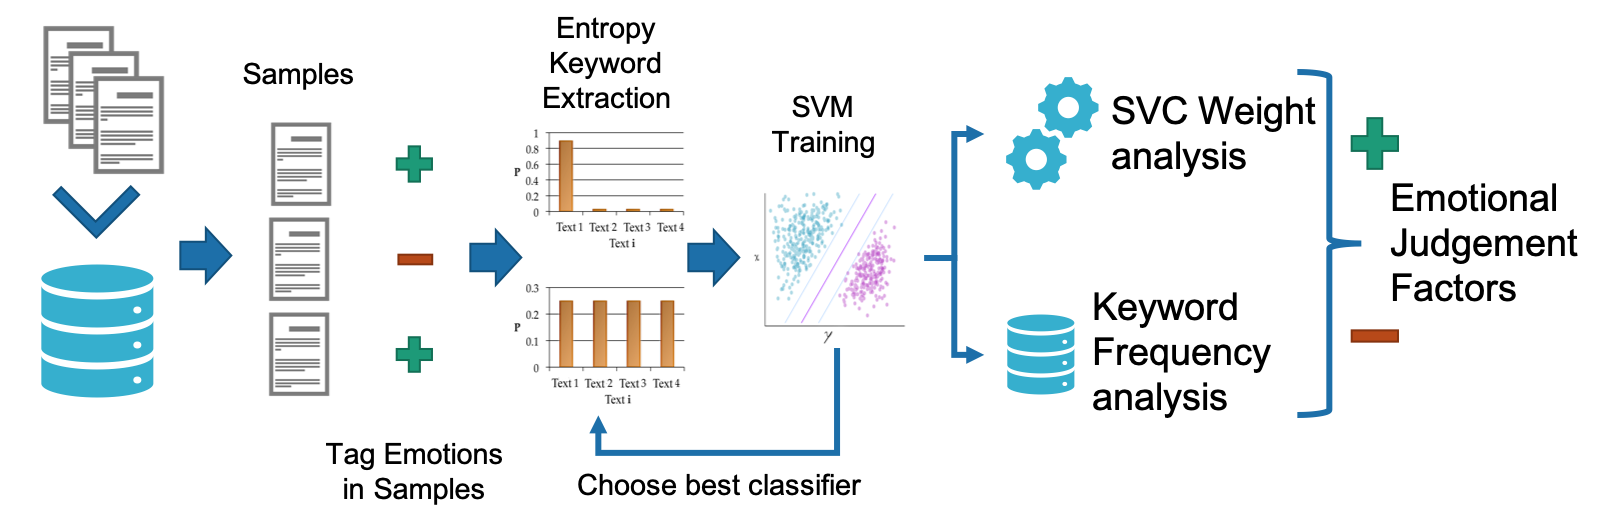
\includegraphics[width=\textwidth]{method-overview.png}
\caption{Overview of the methodology.}
\label{fig:method-overview}
\end{figure}

\subsection{Data collection}\label{datacollection}

In this study we used the HTML parsing python library \textit{BeautifulSoup}\footnote{\label{bs4}Beautiful Soup: \href {https://www.crummy.com/software/BeautifulSoup/}{\path{https://www.crummy.com/software/BeautifulSoup/}}}, and the local database management tool \textit{SQLite}\footnote{\label{sqlite}SQLite: A local database management system with an SQL structure: \href {https://www.sqlite.org/}{\path{https://www.sqlite.org/}}} using the python library \textit{sqlite3} to automatize data managing processes.

\subsection{Data processing}\label{dataprocessing}

\subsubsection{Text processing}\label{textprocessing}

Different from the English language, Chinese texts lack a separation between different words, and as such, when collecting these texts, they are all a single string of characters. To be able to perform a statistical analysis of each word, the Stanford Word Segmenter \cite[][]{chang2008} program developed by the Stanford NLP Group\footnote{\label{stanfordnlp}The Natural Language Processing Group at Stanford University} was implemented for this task using the python \textit{nltk} library. During the segmentation of all the words in our corpus, irregularities occurred where the reviews were written in other languages or where unusual punctuation marks were used. We designated a list of characters that could be recognized as noise, such as punctuation marks, then cleared all the text in the corpus of these characters. 

In the case of texts in English, however, only using spaces is not enough to correctly collect concepts. Because of variations and conjugations of words depending on the context and tense, a better segmentation is achieved by using lemmatization, which returns the dictionary form of each word. For this purpose, we used the \textit{gensim} library with the English texts.

\subsubsection{Sentiment analysis}\label{sentimentanalysis}

\myparagraph{Entropy based keyword extraction}\label{entropy}

In order to determine the words that clearly represent the user’s satisfaction or dissatisfaction, we calculated the entropy value of each word in relation to each class. Shannon’s Entropy, in the field of Information Theory, is defined to be the expected value of the information content in a signal \cite[][]{shannon1948} or it can be thought of as the grade of impossibility of predicting an outcome. It is shown in formulas \ref{eq:H} and \ref{eq:lim_H}. Using this value we can observe the probability distribution of each word inside the corpus. A word that is included in many documents, it will have a high entropy value for that set of documents, since it becomes uncertain to predict in which document it will appear. Opposite to this, a word appearing in only one document will have an entropy value of zero, since it is completely predictable. We show this concept in Figure \ref{fig:entropygraphs}.

\begin{equation}\label{eq:H}
H = - \sum_{i=1}^M [P \log_2 P]
\end{equation}

\begin{equation}\label{eq:lim_H}
\lim_{P\to0+} P \log_2 P = 0
\end{equation}

\begin{figure}[bp]
    \centering
    \begin{subfigure}[b]{0.4\linewidth}
        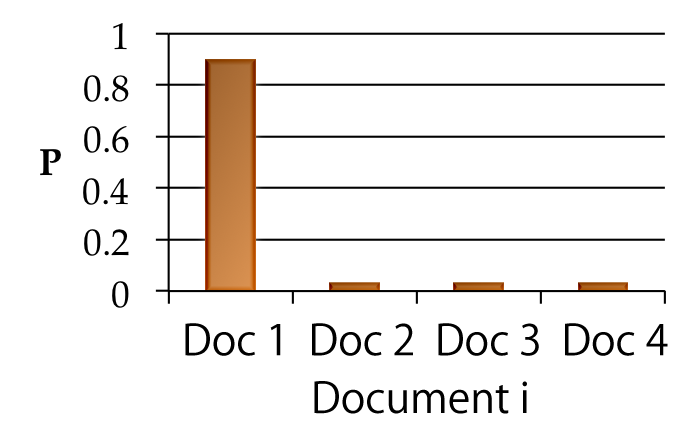
\includegraphics[width=\linewidth]{entropyzero.png}
        \caption{Entropy close to zero.}
    \end{subfigure}
    \begin{subfigure}[b]{0.4\linewidth}
        \includegraphics[width=\linewidth]{entropyhigh.png}
        \caption{High entropy}
    \end{subfigure}
\caption{Probabilities of a word j being contained in a document i.}
\label{fig:entropygraphs}
\end{figure}

To apply this logic, we retrieved 50 reviews as a sample of our corpus and with the collaboration of a group of 5 Chinese students, tagged each sentence of a total of 159 as the classes satisfied or dissatisfied depending on the emotion that the text conveyed, then calculated the entropy values for each word in relation to the set of sentences from each class. In the case of English reviews, we sampled 665 reviews and with the collaboration of English speaking students manually tagged them by sentence, resulting in 2357 tagged sentences. Words with higher entropy relating to the satisfaction set than to the dissatisfaction set by a factor of \(\alpha\) were determined to be keywords tied with satisfaction in Chinese reviews of hotels. This is shown in formula \ref{eq:entropy_pos}. Likewise, words with higher entropy for the dissatisfaction set than the satisfaction set by a factor of \(\alpha'\) were determined to be keywords tied to dissatisfaction in our texts. This is shown in formula \ref{eq:entropy_neg}.

\begin{equation}\label{eq:entropy_pos}
H_{P} > \alpha H_{N} % \rightarrow satisfaction \: keyword
\end{equation}

\begin{equation}\label{eq:entropy_neg}
H_{N} > \alpha' H_{P} % \rightarrow dissatisfaction \: keyword
\end{equation}

\myparagraph{Support Vector Machine classification}\label{svm}

Support Vector Machines are supervised machine learning models usually applied to classification or regression problems \cite[][]{cortes1995}. We use it to classify the rest of our corpus into emotional classes in this study. An SVM is trained to classify data based on previously labeled data, generalizing features of the data by defining a separating (p-1)-dimensional hyperplane in a p-dimensional space in which each dimension is a feature of the data. The separating hyperplane, along with the support vectors, divides the multi-dimensional space and minimize the error of classification. We show a two dimensional example in Figure \ref{fig:svm2d}.

\begin{figure}[bp]
\centering
\includegraphics[width=20em]{SVM_2d_example.png}
\caption{Two dimensional example of an SVM classification problem.}
\label{fig:svm2d}
\end{figure}

In this study, we used the SVM classification process described in \cite[][]{Aleman2018ICAROB} with a number of keyword lists, defined by our entropy calculations with different comparison coefficients, as the possible features; trained the SVMs and tested for each one using a K-fold Cross-Validation method \cite[][]{kohavi1995}. In each test we calculated the Precision, Recall and \(F_1\)-measure \cite[][]{powers2011} for our predictions.


\myparagraph{Model evaluation metrics}
\label{model_evaluation}

In order to measure the effectiveness of the training process and data, we performed what is called K-fold cross-validation. This means that after randomly shuffling and splitting the training data into k equal parts, k-1 of those parts are used for training, while the remaining one part is used in validation. Using the trained models, a prediction is made, and it is decided if such a prediction is correct or not, and counted and grouped as a True Positive, True Negative, False Positive or False Negative prediction. This is explained in Table \ref{tab:preds}.

\begin{table}[bp] \centering
\caption{Prediction outcomes.}\label{tab:preds}
\begin{tabular}{c|c|c|}
\cline{2-3}
\textbf{} & \textbf{Prediction is Correct} & \textbf{Prediction is Incorrect} \\ \hline
\multicolumn{1}{|c|}{\textbf{\begin{tabular}[c]{@{}c@{}}Prediction\\  is Positive\end{tabular}}} & True Positive & False Positive \\ \hline
\multicolumn{1}{|c|}{\textbf{\begin{tabular}[c]{@{}c@{}}Prediction \\ is Negative\end{tabular}}} & True Negative & False Negative \\ \hline
\end{tabular}
\end{table}

Measures of accuracy are determined from these prediction outcomes. This process is then repeated \(k\) times and the measures taken are averaged. In this study, we used the \(F_{1}\) score, which measure is a harmonic mean between precision and recall. Precision, described in formula (\ref{eq:precision}), lets us observe the rate of correct positive predictions from all the positive predictions, while Recall, detailed in formula (\ref{eq:recall}), observes the rate of correct positive predictions from the total of actual positive data. The \(F_{1}\) score in formula (\ref{eq:f1}) then can only be high when both of these measures are high simultaneously and will lower substantially if they are not consistent. We use this score as it allows us to avoid overlooking data while maintaining accurate predictions. The overall accuracy (\ref{eq:accuracy}), which doesn't account for overlooking of data, is also observed for reference but isn't used as the main evaluation of the model.

\begin{equation}\label{eq:precision}
Precision = \frac{True \: Positives}{True \: Positives + False \: Positives}
\end{equation}

\begin{equation}\label{eq:recall}
Recall = \frac{True \: Positives}{True \: Positives + False \: Negatives}
\end{equation}

\begin{equation}\label{eq:f1}
F_{1} = 2  \frac{Precision * Recall}{Precision + Recall}
\end{equation}

\begin{equation}\label{eq:accuracy}
Accuracy = \frac{True \: Positives + True \: Negatives}{Number \: Of \: Predictions}
\end{equation}

\subsubsection{Data analysis}\label{dataanalysis}

\myparagraph{SVM weight analysis}\label{svmweightsanalysis} 

During the SVC learning algorithm, each point of data that is classified incorrectly causes a change in the weight vector to better classify new data correctly. These changes to the weight vector are strong for features that needed to be taken account of to classify with a minimal error, those contained in the support vectors, close to the separating hyperplane. Sequentially, the weight vector can be interpreted as a numerical representation of the effect each feature had for each class in the classification process. Because the weight vector gives value to the words that comprise the support vectors, the words with higher weights are thought to be closer to the dividing hyperplane, while still clearly and decisively belonging to one of the categories the hyperplane divides the high-dimensional space in. While other less ambiguously used words could be excluded from this weight assigning process, the words that are assigned weight values are thought to be words that while discussed in both emotional states, they are more strongly discussed in one of these emotional states. If anything, these are highly volatile words relating to the experience of the customers in the hotel, which are important to consider as a hotel business to improve customer satisfaction. Below we show the formula for the weight vector (\ref{eq:svm_weight}).

\begin{equation}\label{eq:svm_weight}
w = \sum_{i=1}^N \alpha_i y_i x_i
\end{equation}

\myparagraph{Keyword frequency analysis}\label{keywordfrequencyanalysis}

Because the machine learning model used in this study is constructed from training data obtained by a relatively small sample of our data, after training the model and classifying the rest of the data, we studied the frequencies of each entropy based keyword in our complete data set. Words signifying a subject or topic that are relatively highly used will have more meaning when analyzing the emotional response of the user-base of Chinese tourists in Japan.

\section{Results}\label{results}

\subsection{Data set}\label{dataset}

In the data collection stage, a total of \num[group-separator={,}]{1541424} HTML files were crawled, from which 5,938 were unique review pages of hotels in Japan. From these pages, we extracted a total of \num[group-separator={,}]{44912} reviews, which were comprised of 286,109 separate sentences. In our corpus, there were \num[group-separator={,}]{23443} different words used, from which \num[group-separator={,}]{2802} were noise characters.

\subsection{Sentiment analysis results}\label{sentimentresults}

After having the training data tagged by a group of 5 Chinese student collaborators, we experimented with different comparison coefficients for the entropy values calculated from the satisfaction and dissatisfaction emotional classes. The mutually independent coefficients \(\alpha\) and \(\alpha'\) were tested from 1.25 to 6 in intervals of 0.25. The result was 40 lists, 20 for each emotional class. We repeated the process for the reviews in English that our colleagues tagged.

In the beginning, we experimented with different kernels for the SVM, as well as some Ensemble Learning methods, like the Boosting, Voting and Stacking. We ultimately decided to use the linear kernel for the benefits of the weight vector obtainability. We also experimented with different parameters for the SVC, finding that the best performing value for C, a constant that affects the optimization process when minimizing the error of the separating hyperplane. Low values of C give some freedom of error, which minimizes false positives, but depending on the data it can increase false negatives. Inversely, high values of C will likely result in minimal false negatives, but a possibility of false positives. We found the ideal value for this parameter was C=0.5 in our final classifier for Chinese text, and 2 in the English text one.

We trained a different Support Vector Classifier with each of the lists, and we chose the best performing lists for each emotional class, resulting in a satisfaction emotion classifier (satisfied or not) and a dissatisfaction emotion classifier (dissatisfied or not), based on the results of a 5-fold cross-validation process in the Chinese reviews, and a 10-fold cross-validation process in the English reviews case, in which we calculated their accuracy and F-measure means and standard deviations. The number of \(k\)-folds was decided from the sample size. Since the sample for the Chinese texts was smaller, the number of validation data would be reduced if a higher value for \(k\) was used. After observing the misclassification behavior for the satisfaction emotion classifier, which mostly misclassified sentences with negative words, we decided to combine both keyword lists into a single large list to train the satisfaction emotion classifier. With this Combined list, the accuracy was of \(0.92 \pm 0.03\) and \(F_1 = 0.95 \pm 0.01\), both excellent results for classification. Table \ref{tab:svm_f1_zh} shows the lists that had the best performance results in the case of Chinese text and Table \ref{tab:svm_f1_en} shows the best performance results in English texts.

\begin{table}[bp] \centering
\caption{Results of the best 5-fold cross-validation Chinese text classification performance tests.}\label{tab:svm_f1_zh}
\resizebox{\textwidth}{!}{%
\begin{tabular}{|l|l|l|l|l|l|l|}
\hline
Keyword List & \begin{tabular}[c]{@{}l@{}}Classifier \\ emotion\end{tabular} & C & \begin{tabular}[c]{@{}l@{}}Accuracy \\ \(\mu\)\end{tabular} & \begin{tabular}[c]{@{}l@{}}Accuracy\\  \(\sigma\)\end{tabular} & \begin{tabular}[c]{@{}l@{}}\(F_1\) \\ \(\mu\)\end{tabular} & \begin{tabular}[c]{@{}l@{}}\(F_1\) \\ \(\sigma\)\end{tabular} \\ \hline
\begin{tabular}[c]{@{}l@{}}Satisfaction keywords \\ (\(\alpha=2.75\))\end{tabular} & \begin{tabular}[c]{@{}l@{}}Satisfaction \end{tabular} & 2.5 & 0.87 & 0.02 & 0.91 & 0.01 \\ \hline
\begin{tabular}[c]{@{}l@{}}Negative keywords \\ (\(\alpha'=3.75\))\end{tabular} & \begin{tabular}[c]{@{}l@{}}Dissatisfaction \end{tabular} & 0.5 & 0.85 & 0.05 & 0.67 & 0.11 \\ \hline
\begin{tabular}[c]{@{}l@{}}\textbf{Combined} \\ (\(\alpha\)=2.75, \(\alpha'\)=3.75)\end{tabular} & \textbf{\begin{tabular}[c]{@{}l@{}}Satisfaction\end{tabular}} & \textbf{0.5} & \textbf{0.92} & \textbf{0.03} & \textbf{0.95} & \textbf{0.01} \\ \hline
\end{tabular}%
}
\end{table}

\begin{table}[bp] \centering
\caption{Results of the best 10-fold cross-validation English text classification performance tests.}\label{tab:svm_f1_en}
\resizebox{\textwidth}{!}{%
\begin{tabular}{|l|l|l|l|l|l|l|}
\hline
Keyword List & \begin{tabular}[c]{@{}l@{}}Classifier \\ emotion\end{tabular} & C & \begin{tabular}[c]{@{}l@{}}Accuracy \\ \(\mu\)\end{tabular} & \begin{tabular}[c]{@{}l@{}}Accuracy\\  \(\sigma\)\end{tabular} & \begin{tabular}[c]{@{}l@{}}\(F_1\) \\ \(\mu\)\end{tabular} & \begin{tabular}[c]{@{}l@{}}\(F_1\) \\ \(\sigma\)\end{tabular} \\ \hline
\begin{tabular}[c]{@{}l@{}}Satisfaction keywords \\ (\(\alpha=1.5\))\end{tabular} & \begin{tabular}[c]{@{}l@{}}Satisfaction\end{tabular} & 1.75 & 0.79 & 0.02 & 0.82 & 0.02 \\ \hline
\begin{tabular}[c]{@{}l@{}}Dissatisfaction keywords \\ (\(\alpha'=4.25\))\end{tabular} & \begin{tabular}[c]{@{}l@{}}Dissatisfaction\end{tabular} & 3 & 0.70 & 0.04 & 0.80 & 0.03 \\ \hline
\begin{tabular}[c]{@{}l@{}}\textbf{Combined} \\ (\(\alpha\)=1.5, \(\alpha'\)=4.25)\end{tabular} & \textbf{\begin{tabular}[c]{@{}l@{}}Satisfaction\end{tabular}} & \textbf{2} & \textbf{0.81} & \textbf{0.02} & \textbf{0.83} & \textbf{0.02} \\ \hline
\end{tabular}%
}
\end{table}

Using both sets of keywords in the same SVC (named ‘Combined’) to classify the testing data, we obtained higher performance results overall. We then used these classifiers in the rest of the respective data to label positive emotion sentences. The sentences not belonging to the positive emotion class were considered to belong in the negative emotion class since the classification of the emotion of each sentence was binary in our training samples original classification.

\subsection{Keywords and their SVM weight values}\label{svmresults}

In Table \ref{tab:key_weights_zh} we show some of our keywords that signify subjects or topics, and as such, help us understand the needs of the users. We show keywords that have a relatively high weight value for both positive and negative extremes, and their translations in the relevant context. In Table \ref{tab:key_weights_en} we show keywords for the English classifier with high weight values.

\begin{table}[bp] \centering
\caption{High weight values for Chinese keywords signifying subjects or topics.}
\label{tab:key_weights_zh}
\begin{tabular}{|>{\centering\arraybackslash}m{3em}|m{10em}|>{\centering\arraybackslash}m{7em}|>{\centering\arraybackslash}m{5em}|} \hline
\textbf{Word} & \multicolumn{1}{c|}{\textbf{Translation}} & \textbf{Entropy List} & \textbf{SVC Weight} \\ \hline
\begin{CJK}{UTF8}{gbsn} 地方 \end{CJK} 
    & region, local 
        & Satisfaction 
        & 1.343 \\ \hline
\begin{CJK}{UTF8}{gbsn} 干净 \end{CJK} 
    & clean 
        & Satisfaction 
        & 0.638 \\ \hline
\begin{CJK}{UTF8}{gbsn} 大 \end{CJK} 
    & big, wide 
        & Satisfaction 
        & 0.624 \\ \hline
\begin{CJK}{UTF8}{gbsn} 交通 \end{CJK} 
    & traffic, transportation 
        & Satisfaction 
        & 0.586 \\ \hline
\begin{CJK}{UTF8}{gbsn} 热情 \end{CJK} 
    & cordial, kindness 
        & Satisfaction 
        & 0.495 \\ \hline
\begin{CJK}{UTF8}{gbsn} 周边 \end{CJK} 
    & periphery 
        & Satisfaction 
        & 0.495 \\ \hline
\begin{CJK}{UTF8}{gbsn} 景色 \end{CJK} 
    & scenery 
        & Satisfaction 
        & 0.495 \\ \hline
\begin{CJK}{UTF8}{gbsn} 推荐 \end{CJK} 
    & recommendation 
        & Satisfaction 
        & 0.495 \\ \hline
\begin{CJK}{UTF8}{gbsn} 日本 \end{CJK} 
    & Japan 
        & Satisfaction 
        & 0.495 \\ \hline
\begin{CJK}{UTF8}{gbsn} 早餐 \end{CJK} 
    & breakfast 
        & Satisfaction 
        & 0.495 \\ \hline
\begin{CJK}{UTF8}{gbsn} 附近 \end{CJK} 
    & nearby 
        & Satisfaction 
        & 0.495 \\ \hline
\begin{CJK}{UTF8}{gbsn} 中文 \end{CJK} 
    & Chinese text 
        & Dissatisfaction 
        & -0.714 \\ \hline
\begin{CJK}{UTF8}{gbsn} 地理 \end{CJK} 
    & geography 
        & Dissatisfaction 
        & -0.812 \\ \hline
\begin{CJK}{UTF8}{gbsn} 价格 \end{CJK} 
    & price 
        & Dissatisfaction 
        & -1.505 \\ \hline
\end{tabular}
\end{table}

\begin{table}[bp]
\centering
\caption{High weight values for English keywords signifying subjects or topics.}
\label{tab:key_weights_en}
\begin{tabular}{|l|c|c|}
\hline
\multicolumn{1}{|c|}{\textbf{Word}} & \multicolumn{1}{c|}{\textbf{\begin{tabular}[c]{@{}c@{}}Entropy\\ List\end{tabular}}} & \multicolumn{1}{c|}{\textbf{SVC Weight}} \\ \hline
bathhouse & Satisfaction & 2.000 \\ \hline
museum & Satisfaction & 2.000 \\ \hline
meeting & Satisfaction & 1.997 \\ \hline
subway & Satisfaction & 1.951 \\ \hline
cozy & Satisfaction & 2.000 \\ \hline
convenience & Satisfaction & 1.888 \\ \hline
clean & Satisfaction & 1.886 \\ \hline
comfortable & Satisfaction & 1.724 \\ \hline
dirty & Dissatisfaction & -1.275 \\ \hline
policy & Dissatisfaction & -1.463 \\ \hline
prepay & Dissatisfaction & -1.517 \\ \hline
pricey & Dissatisfaction & -1.614 \\ \hline
sticky & Dissatisfaction & -2.000 \\ \hline
\end{tabular}
\end{table}

\subsection{Keyword frequencies}\label{freqresults}

We observed the words with the highest frequencies for keywords in satisfied and dissatisfied statements to study and quantitatively rank the needs of Chinese customers, as shown in the Tables \ref{tab:pos_keys_zh} and \ref{tab:neg_keys_zh}; and for English speaking customers, as shown in Tables \ref{tab:pos_keys_en} and \ref{tab:neg_keys_en}.

\begin{table}[bp] \centering
\caption{High weight Chinese keywords in satisfaction sentences.}
\label{tab:pos_keys_zh}
\begin{tabular}{|c|l|c|c|} \hline
\textbf{Word} & \multicolumn{1}{c|}{\textbf{Translation}} & \textbf{Frequency} & \textbf{SVC Weight} \\ \hline
\begin{CJK}{UTF8}{gbsn} 大 \end{CJK} 
    & big 
        & 15470 & 0.624 \\ \hline
\begin{CJK}{UTF8}{gbsn} 干净 \end{CJK} 
    & clean 
        & 12166 & 0.638 \\ \hline
\begin{CJK}{UTF8}{gbsn} 早餐 \end{CJK} 
    & breakfast 
        & 10575 & 0.495 \\ \hline
\begin{CJK}{UTF8}{gbsn} 推荐 \end{CJK} 
    & recommendation 
        & 8752 & 0.495 \\ \hline
\begin{CJK}{UTF8}{gbsn} 环境 \end{CJK} 
    & \begin{tabular}[c]{@{}l@{}}
    environment, \\ surroundings 
    \end{tabular} 
        & 8694 & 0.248 \\ \hline
\end{tabular}
\end{table}


\begin{table}[bp] \centering
\caption{High negative weight Chinese keywords in dissatisfaction sentences.}
\label{tab:neg_keys_zh}
\begin{tabular}{|c|l|c|c|} \hline
\textbf{Word} & \multicolumn{1}{c|}{\textbf{Translation}} & \textbf{Frequency} & \textbf{SVC Weight} \\ \hline
\begin{CJK}{UTF8}{gbsn} 价格 \end{CJK} 
    & price & 7636 & -1.505 \\ \hline
\begin{CJK}{UTF8}{gbsn} 地理 \end{CJK} 
    & geography & 2238 & -0.812 \\ \hline
\begin{CJK}{UTF8}{gbsn} 中文 \end{CJK} 
    & Chinese language & 1410 & -0.714 \\ \hline
\end{tabular}
\end{table}

\begin{table}[bp]
\centering
\caption{High weight English keywords in satisfaction sentences.}
\label{tab:pos_keys_en}
\begin{threeparttable}
\begin{tabular}{|l|c|c|}
\hline
\multicolumn{1}{|c|}{\textbf{Word}} & \textbf{Frequency} & \textbf{SVC Weight} \\ \hline
staff & 138677 & 0.537 \\ \hline
clean & 105971 & 1.886 \\ \hline
location & 103151 & 0.842 \\ \hline
comfortable & 62793 & 1.724 \\ \hline
subway & 38354 & 1.951 \\ \hline
airport & 36328 & 0.839 \\ \hline
shopping & 34355 & 1.308 \\ \hline
onsen \tnote{*} & 31084 & 0.094 \\ \hline
\end{tabular}
\begin{tablenotes}
\item[*]Onsen are Japanese hot springs
\end{tablenotes}
\end{threeparttable}
\end{table}

\begin{table}[bp]
\centering
\caption{High negative weight English keywords in dissatisfaction sentences.}
\label{tab:neg_keys_en}
\begin{tabular}{|l|c|c|}
\hline
\multicolumn{1}{|c|}{\textbf{Word}} & \textbf{Frequency} & \textbf{SVC Weight} \\ \hline
pricey & 3809 & -1.614 \\ \hline
carpet & 3683 & -0.507 \\ \hline
dirty & 2943 & -1.275 \\ \hline
stain & 2787 & -1.886 \\ \hline
cigarette & 2468 & -0.435 \\ \hline
\end{tabular}
\end{table}

In order to further analyze the data we obtained, aside from emotional classification, we also investigated the difference in emotional response from customers of hotels in different price brackets in the case of Chinese reviews. We separated hotel prices in 6 categories, and in Table \ref{tab:keys_prices} we show the words that have an interesting change in their ranking order when ordered by frequency in each price bracket. We include the price bracket definitions in \ref{appendix:price_ranges} in Table \ref{tab:price_ranges}.


\begin{table}[bp] \centering
\caption{Words that change in importance between price brackets in positive sentences.}
\label{tab:keys_prices}
\begin{tabular}{|>{\centering\arraybackslash}m{2.5em}|m{6em}|m{16em}|} \hline
\multicolumn{1}{|c|}{\textbf{Word}} & \multicolumn{1}{c|}{\textbf{Translation}} & \multicolumn{1}{c|}{\textbf{Observation}} \\ \hline
\begin{CJK}{UTF8}{gbsn} 交通 \end{CJK}
    & \begin{tabular}[c]{@{}l@{}}traffic,\\ transportation \end{tabular} 
        & Higher ranking for hotels with lower prices, while not as high in luxury hotels. \\ \hline
\begin{CJK}{UTF8}{gbsn} 环境 \end{CJK} 
    & \begin{tabular}[c]{@{}l@{}}environment,\\ surroundings \end{tabular} 
        & Higher ranking for luxury hotels and in the lowest priced hotels, but not as high in the middle price brackets. \\ \hline
\begin{CJK}{UTF8}{gbsn} 日式 \end{CJK} 
    & japanese-style 
        & Only high ranking in luxury hotels. \\ \hline
\begin{CJK}{UTF8}{gbsn} 人员 \end{CJK} 
    & \begin{tabular}[c]{@{}l@{}}staff,\\ personnel \end{tabular} 
        & Rises in ranking as the hotel price rises. \\ \hline
\begin{CJK}{UTF8}{gbsn} 推荐 \end{CJK} 
    & recommend 
        & Included in all hotels, but higher ranking in lower priced hotels. \\ \hline
\end{tabular}
\end{table}

\section{Discussion}\label{discussion}

\subsection{Needs of the Chinese tourist market in Japan}\label{discussionneeds}

Analyzing the results from the extracted keywords is the key to understanding Chinese and English speaking customers of Japanese hotels since they can be interpreted as rankings of their explicit needs and demands. Analyzing satisfaction keywords, we found that the most relevant subjects Chinese customers perceive positively are cleanliness and size, very possibly of the room they had stayed in. There is also the possibility that reviewers were praising, in general, the cleanliness of Japan’s environment, un-littered streets, potable water and their culture of respecting spaces. Our results are compatible with \cite{ryan2001} in their study of Chinese tourist behavior in New Zealand , where Chinese travelers were found to prefer traveling and exploring unfamiliar places that have a reputation for being clean and unpolluted environments, focusing on scenic beauty, history and culture. They also found complaints about the lack of Chinese language availability in the services they consumed. \cite{LIU2019337} describe that the behavior studied in Australia reflected that Chinese tourists were more likely to appreciate touristic places for the scenery, architecture, landmarks, and popular spots, rather than appreciate cultural experiences or activities. Similar to the findings in Liu et al., our results indicate that closeness of the hotel to scenic places is highly tied to satisfaction. However, their research is on online reviews of touristic places, instead of hotels. With this difference, our results showed that breakfast inclusion and the size and cleanliness of rooms were also tied to satisfaction, aside from scenery. According to our data, other positive factors that come into play when Chinese tourists choose a hotel to stay is the location in relation to public transport availability; and as mentioned before, environments, such as gardens or parks nearby; and services nearby, like places to go shopping. \cite{gao2017chinese} argue that Chinese people are heavily influenced by religion and a culture that regards harmony and oneness with nature and humans, which in turn influences their tourism behavior. However, they also argue that there are generational differences and that the older generations that lived through the changes that changed the environment and caused pollution care more about the environment, and as such appreciate natural and scenic touristic spots more than younger generations.

One key component we found in Chinese customer satisfaction is the inclusion of breakfast within the hotel. This can be inferred from the high frequency with which this keyword was included in the sentences emotionally classified as positive. While other food-related words were extracted, most of them were general in nature, like “food” or “eating”, and in a lower ranking. In contrast, the word “breakfast”, which is referring to a specific time and very possibly its inclusion in the hotel commodities, was very frequently used in positive texts compared to other food-related words. This specific keyword is previously unmentioned in studies regarding the eating behavior of Chinese tourists. While these studies on eating behavior are very scarce, both a study on the food preferences of Chinese tourists in Australia \cite[][]{chang2010} and an article on Chinese food culture \cite[][]{ma2015} state that even in foreign countries, Chinese people have a habit to eat Chinese food, probably because of a need for familiarity. However, the analysis of our data points to the fact that more than Chinese food as a specific concept, hotel reviews are written with general words that represent food. We would like to further study specific Chinese tourists food preferences, such as the contents of said breakfast and other meals in future work to observe the level of necessity of these particular needs.

Now, when analyzing dissatisfied responses, the most frequently criticized aspect of Japanese hotels was the price. This was true across all of the price brackets, from the cheapest hotels to the most luxurious ones. In their study of Chinese tourists in Vietnam, \cite{truong2009} also found both the tendency to be concerned with value for money. It is possible that concerns over value for money are a general cultural trait in the Chinese population. Applying this previous finding to our data, negativity about the pricing of hotels across all price brackets can mean they believe the price is too high for the service that they receive, regardless of their satisfaction or dissatisfaction with the service. Our results suggest that Chinese customers are expecting lower prices for whatever services they receive.  

Another important negative factor can be the availability or lack thereof of Chinese translations. Chinese customers can feel lost when they don't understand directions or instructions, either written or spoken; however, according to our data, most customers can be thought to have complained about written translations. 

Additionally, as shown in Table \ref{tab:keys_prices}, there is a positive reaction to “Japanese-style”, which we infer in this context can mean rooms or possibly ceremonies, in luxury rate hotels. Another interesting point is that the expectation for hotel staff increases as the price of the hotel rises. Furthermore, while “recommendation” of a hotel can be seen across all price brackets, customers searching for low priced hotels are relatively more inclined to recommend that hotel to others, based on a comparison of frequency ranking of each word for each price bracket.

\subsection{Comparison with English speaking tourists in Japan}

The results with the English speaking population are similar to the results with the Chinese speaking population, but there are some noteworthy differences that can be explored. For example, while Chinese customers seem to focus positively on the cleanliness of the room first and foremost, English speaking customers seem to consider the behavior of the staff before it. However, when we consider the negative associations, the price is the first concern for both kinds of customers, but there's a high concern for cleanliness in a negative connotation, such as complaints about stains, dirty rooms or carpets. A thing to note is that there is a high number of complaints about cigarette smell, in comparison to the Chinese customers in which it isn't a keyword within our extraction methods. Previous research states that 49 - 60\% of Chinese men (and 2.0 - 2.8\% of women) currently smoke or have smoked before, taken from a sample of \num[group-separator={,}]{170000} Chinese adults in 2013-2014, which is high compared to many English speaking countries \cite[][]{zhang2019tobacco, who2015tobacco}. 

In previous research, it has been found that Chinese tourists are harsher in their negative touristic attraction reviews than other nationalities \cite[][]{LIU2019337}. Taking this into account, and the large difference in frequency between complaints about price and other elements, Chinese customers can be said to be dissatisfied with price in a disproportionate way. English speaking tourists' dissatisfaction factors, on the other hand, have less of a gap in frequency, and as such can be said to be more concerned about cleanliness related factors than price.

On the positive reviews side, there is a high number of mentions for nearby transportation methods, such as the subway, or access from the airport. This is also different when compared to Chinese customers, who don't mention transportation services as frequently for viewing a hotel in a positive way. Another difference that is noteworthy is that Chinese customers appreciate included breakfast in hotels, but for the English speaking customers it seems to not be a priority.

\section{Conclusions and future work}\label{conclusions}

In this study, with the purpose to understand emotional responses of Chinese customers of Japanese hotels and understand their needs, we extracted keywords from their reviews from the Chinese portal site \textit{Ctrip} using entropy calculations from a manually classified sample of our data; then we used these keywords in machine learning experiments. Using the keywords to train a linear kernel Support Vector Classifier, we obtained the highest performance \((F=0.95\pm0.01\) and \(Accuracy = 0.92\pm0.03)\) using both our positive and negative keywords for a binary emotional classifier.

Using the weight vectors of our classifiers, as well as frequency of the words in our dataset, we found that Chinese customers have a preference for big and clean rooms, big thermal baths or bathhouses, expect good value for money regardless of price, that there is a lack of Chinese text translation and that they prefer hotels where breakfast is included. We also found that the friendliness of the staff increases in priority as the price and luxury of the hotel increases and that transportation is more important for customers looking for cheaper options compared to the more luxurious ones.

For comparison, we also repeated the experiments on reviews written by English speaker tourists staying at Japanese hotels from \textit{TripAdvisor}. Observing the results we identified that English speaking customers hold a bigger contempt and negative reactions for dirty or stained rooms, but that the main concern is also the pricing of the hotels. We also found that they prefer friendly staff and transportation available from the airport or subway.

Our results show the needs of a large and increasing segment of the customers. This would have otherwise presented difficulties with traditional methods because of language and culture barriers. The hotel industry can make use of these results to better the response from Chinese customers by focusing on improving topics they find important, such as cleanliness, the inclusion of breakfast, availability of Chinese translations in text format and so on. By doing this, satisfied users will write new reviews and thus influence future customers positively.

In future work we plan to investigate further into this topic, extending our data set and researching for different trends for different regions of Japan and in different kinds of hotels, as well as between customers traveling alone or in groups, for fun or for work. Another point for the future of this study is to use word clusters with similar meanings instead of single words. As mentioned before, we would also study the food preferences of Chinese tourists, as well as the impact of the recommendation in different price brackets. Additionally, it would be interesting to study further into more specific emotions than the satisfaction and dissatisfaction classifications we performed in our study.

\section*{Acknowledgements}

During our research, apart from the group of Chinese students that collaborated with the training data and emotion tagging process, we received the commentary and discussion necessary to understand certain
cultural aspects that could influence the interpretation of the data, from empirical and anecdotal Chinese sources, as well as collaboration in understanding the meaning behind the words we extracted by our dear colleagues, whom we would like to show gratitude to, Mr. Zhou Liangyuan, Ms. Eerdengqiqige, and Mr. Hugo Alberto Mendoza España.

\medskip

Funding: This work was supported by the Japan Construction Information Center Foundation (JACIC).

\medskip

Declarations of interest: none

\clearpage
\section*{References}

\bibliography{mybibfile}

\clearpage

\appendixpage
\appendix

\section{Price bracket analysis details}\label{appendix:price_ranges}

In the Keyword Frequency Analysis in section \ref{freqresults} and Table \ref{tab:keys_prices}, we examined the frequency of certain keywords across different price brackets. We show these ranges in Table \ref{tab:price_ranges}. These price brackets were selected by observing different kinds of hotels and their level of luxury, along with their price. Hostels and capsule hotels depending on their location are often in the first two price brackets. Business hotels can range from the third to fourth, while more luxurious hotels are included in the fifth and sixth ranges. The price data was mined as the average price per night in a hotel using the data available in \textit{Ctrip}, and not for each review as it might vary by the number of nights and the kind of room chosen.

\begin{table}[hbp] \centering
\caption{Price per night ranges used for analysis.}\label{tab:price_ranges}
\begin{tabular}{|l|l|}
\hline
\multicolumn{1}{|c|}{\textbf{Price bracket Number}} & \multicolumn{1}{c|}{\textbf{Price bracket in japanese yen}} \\ \hline
Price Bracket 1 & 0 yen to 5000 yen \\ \hline
Price Bracket 2 & 5000 yen to 10,000 yen \\ \hline
Price Bracket 3 & 10,000 yen to 15,000 yen \\ \hline
Price Bracket 4 & 15,000 yen to 20,000 yen \\ \hline
Price Bracket 5 & 20,000 yen to 100,000 yen \\ \hline
Price Bracket 6 & 100,000 yen to 500,000 yen \\ \hline
\end{tabular}
\end{table}

\end{document}
